% !TeX root = tcolorbox.tex
% include file of tcolorbox.tex (manual of the LaTeX package tcolorbox)
\clearpage
\section{Library \mylib{vignette}}\label{sec:vignette}%
\tcbset{external/prefix=external/vignette_}%
The library is loaded by a package option or inside the preamble by:
\begin{dispListing}
\tcbuselibrary{vignette}
\end{dispListing}
This also loads the \mylib{skins} library, see \zvref[S]{sec:skins},
and the |fadings| library of |tikz| \cite{tantau:tikz_and_pgf}.


\subsection{Vignette Drawing}\label{subsec:vignettedrawing}

\begin{docCommand}[doc new=2016-04-22]{tcbvignette}{\marg{options}}
  In this context, a \emph{vignette} is a four part rectangular frame.
  It is constructed as several \tikzname\ paths and, therefore, can only be
  used inside a |tikzpicture| environment or inside \refEnv{tcolorbox} options.

  The \meta{options} control position, size and style settings of the vignette.
  Theses options have the common key path |/tcb/vig/| and are described in
  the following.

  The next examples show direct \refCom{tcbvignette} usage without
  a \refEnv{tcolorbox}.

\begin{dispExample*}{sbs,righthand width=3cm,center lower}
\begin{tikzpicture}
  \tcbvignette{}
\end{tikzpicture}
\end{dispExample*}

\begin{dispExample*}{sbs,righthand width=3cm,center lower}
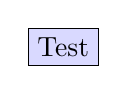
\begin{tikzpicture}
  \node[draw,fill=blue!15!white] (A) {Test};
  \tcbvignette{outside node=A,raised color=blue}
\end{tikzpicture}
\end{dispExample*}

\begin{dispExample*}{sbs,righthand width=3cm,center lower}
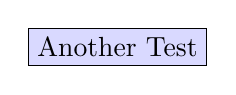
\begin{tikzpicture}
  \node[draw,fill=blue!15!white] (A) {Another Test};
  \tcbvignette{size=3mm,outside node=A,
    north style=red,east style=yellow,
    south style=blue,west style=green}
\end{tikzpicture}
\end{dispExample*}

\begin{dispExample*}{sbs,righthand width=3cm,center lower}

\begin{tikzpicture}
  \node[inner sep=3mm,fill=red!75] (A) {Test};
  \tcbvignette{over node=A,fade in}
\end{tikzpicture}
\end{dispExample*}

\refCom{tcbvignette} can be used directly inside appropriate options keys
for \refEnv{tcolorbox}. Note that options like \refKey{/tcb/underlay} need
\refKey{/tcb/enhanced} or similar settings.

\begin{dispExample*}{sbs,righthand width=3cm,center lower}
\begin{tcolorbox}[enhanced,size=small,sharp corners,
  colback=green!10,colframe=green!50!black,
  boxrule=1mm,titlerule=0mm,
  title=My title,center title,fonttitle=\bfseries,
  underlay={\tcbvignette{size=1mm,inside node=frame,
      raised color=green!50!black}}]
    This is a tcolorbox.
\end{tcolorbox}
\end{dispExample*}

Mostly, convenient short cuts like \refKey{/tcb/underlay vignette} can
be used to add a \emph{vignette} to a \refEnv{tcolorbox}. Here, \refCom{tcbvignette}
is used internally.

\begin{dispExample*}{sbs,righthand width=3cm,center lower}
\begin{tcolorbox}[enhanced,size=small,sharp corners,
  colback=green!10,colframe=green!50!black,
  boxrule=1mm,titlerule=0mm,
  title=My title,center title,fonttitle=\bfseries,
  underlay vignette]
    This is a tcolorbox.
\end{tcolorbox}
\end{dispExample*}

\end{docCommand}



\subsection{Generic Geometry Settings}\label{subsec:vignettegeometry}


\begin{vigTcbKey}[][doc new=2016-04-22]{xmin}{=\meta{length}}{no default, initially |0pt|}
  Sets the lower horizontal limit of a \refCom{tcbvignette}.
\end{vigTcbKey}

\begin{vigTcbKey}[][doc new=2016-04-22]{xmax}{=\meta{length}}{no default, initially |1cm|}
  Sets the upper horizontal limit of a \refCom{tcbvignette}.
\end{vigTcbKey}

\begin{vigTcbKey}[][doc new=2016-04-22]{ymin}{=\meta{length}}{no default, initially |0pt|}
  Sets the lower vertical limit of a \refCom{tcbvignette}.
\end{vigTcbKey}

\begin{vigTcbKey}[][doc new=2016-04-22]{ymax}{=\meta{length}}{no default, initially |1cm|}
  Sets the upper vertical limit of a \refCom{tcbvignette}.
\end{vigTcbKey}


\begin{dispExample*}{sbs,righthand width=3cm,center lower}
\begin{tikzpicture}
  \fill [black!20] (0,0) rectangle (3,2);
  \path [pattern=checkerboard,pattern color=black!30]
    (0,0) rectangle (3,2);
  \tcbvignette{xmin=1cm,xmax=2.5cm,ymin=0.5cm,ymax=1.75cm}
\end{tikzpicture}
\end{dispExample*}


\begin{vigTcbKey}[][doc new=2016-04-22]{lower left corner}{=\meta{coordinates}}{style, initially |0,0|}
  Sets the lower left corner of a \refCom{tcbvignette}.
  This style sets \refKey{/tcb/vig/xmin} and \refKey{/tcb/vig/ymin}.
\end{vigTcbKey}

\begin{vigTcbKey}[][doc new=2016-04-22]{upper right corner}{=\meta{coordinates}}{style, initially |1,1|}
  Sets the upper right corner of a \refCom{tcbvignette}.
  This style sets \refKey{/tcb/vig/xmax} and \refKey{/tcb/vig/ymax}.
\end{vigTcbKey}


\begin{dispExample*}{sbs,righthand width=3cm,center lower}
\begin{tikzpicture}
  \fill [black!20] (0,0) rectangle (3,2);
  \path [pattern=checkerboard,pattern color=black!30]
    (0,0) rectangle (3,2);
  \tcbvignette{lower left corner={1,0.5},
               upper right corner={2.5,1.75}}
\end{tikzpicture}
\end{dispExample*}

\enlargethispage*{1cm}

\begin{vigTcbKey}[][doc new=2016-04-22]{inside node}{=\meta{name}}{style, initially unset}
  Places the \refCom{tcbvignette} inside the node with the given \meta{name}.
  The outer limits of the \emph{vignette} are adapted to the node geometry.
\begin{dispExample*}{sbs,righthand width=3cm,center lower}
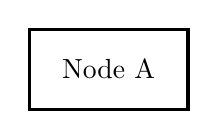
\begin{tikzpicture}
  \node[minimum width=2cm,minimum height=1cm] (A) {Node A};
  \tcbvignette{inside node=A}
  \draw[very thick] (A.south west) rectangle (A.north east);
\end{tikzpicture}
\end{dispExample*}
\end{vigTcbKey}

\clearpage

\begin{vigTcbKey}[][doc new=2016-04-22]{outside node}{=\meta{name}}{style, initially unset}
  Places the \refCom{tcbvignette} outside the node with the given \meta{name}.
  The inner limits of the \emph{vignette} are adapted to the node geometry.
\begin{dispExample*}{sbs,righthand width=3cm,center lower}
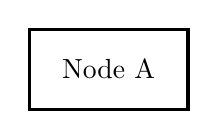
\begin{tikzpicture}
  \node[minimum width=2cm,minimum height=1cm] (A) {Node A};
  \tcbvignette{outside node=A}
  \draw[very thick] (A.south west) rectangle (A.north east);
\end{tikzpicture}
\end{dispExample*}
\end{vigTcbKey}


\begin{vigTcbKey}[][doc new=2016-04-22]{over node}{=\meta{name}}{style, initially unset}
  Places the \refCom{tcbvignette} over the node with the given \meta{name}.
  The outer limits of the \emph{vignette} are adapted to the node geometry, but
  are shifted to the outside by \refKey{/tcb/vig/over node offset}.
\begin{dispExample*}{sbs,righthand width=3cm,center lower}
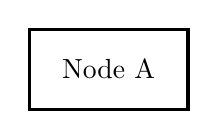
\begin{tikzpicture}
  \node[minimum width=2cm,minimum height=1cm] (A) {Node A};
  \tcbvignette{over node offset=1mm,over node=A}
  \draw[very thick] (A.south west) rectangle (A.north east);
\end{tikzpicture}
\end{dispExample*}
\end{vigTcbKey}

\begin{vigTcbKey}[][doc new=2016-04-22]{over node offset}{=\meta{length}}{no default, initially |0.1mm|}
  Determines the shift value for \refKey{/tcb/vig/over node}.
  Note that \refKey{/tcb/vig/over node offset} has to be set \emph{before}
  \refKey{/tcb/vig/over node} is used.
\end{vigTcbKey}


\begin{vigTcbKey}[][doc new=2016-04-22]{north size}{=\meta{length}}{no default, initially |2mm|}
  Sets the thickness of the north \emph{vignette} part.
\begin{dispExample*}{sbs,righthand width=3cm,center lower}
\begin{tikzpicture}
  \tcbvignette{north size=4mm}
\end{tikzpicture}
\end{dispExample*}
\end{vigTcbKey}

\begin{vigTcbKey}[][doc new=2016-04-22]{south size}{=\meta{length}}{no default, initially |2mm|}
  Sets the thickness of the south \emph{vignette} part.
\begin{dispExample*}{sbs,righthand width=3cm,center lower}
\begin{tikzpicture}
  \tcbvignette{south size=4mm}
\end{tikzpicture}
\end{dispExample*}
\end{vigTcbKey}

\begin{vigTcbKey}[][doc new=2016-04-22]{east size}{=\meta{length}}{no default, initially |2mm|}
  Sets the thickness of the east \emph{vignette} part.
\begin{dispExample*}{sbs,righthand width=3cm,center lower}
\begin{tikzpicture}
  \tcbvignette{east size=4mm}
\end{tikzpicture}
\end{dispExample*}
\end{vigTcbKey}

\begin{vigTcbKey}[][doc new=2016-04-22]{west size}{=\meta{length}}{no default, initially |2mm|}
  Sets the thickness of the west \emph{vignette} part.
\begin{dispExample*}{sbs,righthand width=3cm,center lower}
\begin{tikzpicture}
  \tcbvignette{west size=4mm}
\end{tikzpicture}
\end{dispExample*}
\end{vigTcbKey}

\clearpage

\begin{vigTcbKey}[][doc new=2016-04-22]{vertical size}{=\meta{length}}{style, initially |2mm|}
  Sets \refKey{/tcb/vig/north size} and \refKey{/tcb/vig/south size},
  to the given \meta{length}.
\begin{dispExample*}{sbs,righthand width=3cm,center lower}
\begin{tikzpicture}
  \tcbvignette{vertical size=4mm}
\end{tikzpicture}
\end{dispExample*}
\end{vigTcbKey}

\begin{vigTcbKey}[][doc new=2016-04-22]{horizontal size}{=\meta{length}}{style, initially |2mm|}
  Sets \refKey{/tcb/vig/east size} and \refKey{/tcb/vig/west size},
  to the given \meta{length}.
\begin{dispExample*}{sbs,righthand width=3cm,center lower}
\begin{tikzpicture}
  \tcbvignette{horizontal size=4mm}
\end{tikzpicture}
\end{dispExample*}
\end{vigTcbKey}


\begin{vigTcbKey}[][doc new=2016-04-22]{size}{=\meta{length}}{style, initially |2mm|}
  Sets \refKey{/tcb/vig/north size}, \refKey{/tcb/vig/south size},
  \refKey{/tcb/vig/east size}, and \refKey{/tcb/vig/west size} to the given \meta{length}.
\begin{dispExample*}{sbs,righthand width=3cm,center lower}
\begin{tikzpicture}
  \tcbvignette{size=4mm}
\end{tikzpicture}
\end{dispExample*}
\end{vigTcbKey}


\begin{marker}
\refKey{/tcb/vig/north size}, \refKey{/tcb/vig/south size}, etc. have to
be set \emph{before} \refKey{/tcb/vig/outside node} is used.
\end{marker}



\subsection{Generic Color and Style Settings}\label{subsec:vignettestyle}

\begin{vigTcbKey}[][doc new=2016-04-22]{north style}{=\marg{style}}{no default, initially |red!50!white|}
  Sets \tikzname\ \meta{style} options for the north \emph{vignette} part.
\begin{dispExample*}{sbs,righthand width=3cm,center lower}
\begin{tikzpicture}
  \tcbvignette{north style=blue}
\end{tikzpicture}
\end{dispExample*}
\end{vigTcbKey}

\begin{vigTcbKey}[][doc new=2016-04-22]{south style}{=\marg{style}}{no default, initially |red!50!black|}
  Sets \tikzname\ \meta{style} options for the south \emph{vignette} part.
\begin{dispExample*}{sbs,righthand width=3cm,center lower}
\begin{tikzpicture}
  \tcbvignette{south style={draw=blue,fill=yellow}}
\end{tikzpicture}
\end{dispExample*}
\end{vigTcbKey}


\begin{vigTcbKey}[][doc new=2016-04-22]{east style}{=\marg{style}}{no default, initially |red!75!black|}
  Sets \tikzname\ \meta{style} options for the east \emph{vignette} part.
\begin{dispExample*}{sbs,righthand width=3cm,center lower}
\begin{tikzpicture}
  \tcbvignette{east style={left color=yellow!75!black,
    right color=blue!75!black}}
\end{tikzpicture}
\end{dispExample*}
\end{vigTcbKey}

\clearpage

\begin{vigTcbKey}[][doc new=2016-04-22]{west style}{=\marg{style}}{no default, initially |red!75!white|}
  Sets \tikzname\ \meta{style} options for the west \emph{vignette} part.
\begin{dispExample*}{sbs,righthand width=3cm,center lower}
\begin{tikzpicture}
  \tcbvignette{west style={preaction={fill=black!20},
    pattern=checkerboard,
    pattern color=black!30}}
\end{tikzpicture}
\end{dispExample*}
\end{vigTcbKey}


\begin{vigTcbKey}[][doc new=2016-05-24]{scope}{=\marg{style}}{no default, initially empty}
  The four \emph{vignette} parts are drawn inside a \tikzname\ |scope|
  environment which takes the given \meta{style} as option.
\begin{dispExample*}{sbs,righthand width=3cm,center lower}
\begin{tikzpicture}
  \tcbvignette{scope={transparency group,opacity=0.25}}
\end{tikzpicture}
\end{dispExample*}
\end{vigTcbKey}



\begin{vigTcbKey}[][doc new=2016-04-22]{raised color}{=\meta{color}}{no default}
  Creates a raised frame impression by setting the four style options
  \refKey{/tcb/vig/north style},
  \refKey{/tcb/vig/south style},
  \refKey{/tcb/vig/east style}, and
  \refKey{/tcb/vig/west style}
  to darkened and lightened variations of the given \meta{color}.
\begin{dispExample*}{sbs,righthand width=3cm,center lower}
\begin{tikzpicture}
  \tcbvignette{raised color=blue}
\end{tikzpicture}
\end{dispExample*}
\end{vigTcbKey}


\begin{vigTcbKey}[][doc new=2016-04-22]{lowered color}{=\meta{color}}{no default}
  Creates a lowered frame impression by setting the four style options
  \refKey{/tcb/vig/north style},
  \refKey{/tcb/vig/south style},
  \refKey{/tcb/vig/east style}, and
  \refKey{/tcb/vig/west style}
  to darkened and lightened variations of the given \meta{color}.
\begin{dispExample*}{sbs,righthand width=3cm,center lower}
\begin{tikzpicture}
  \tcbvignette{lowered color=green!75!black}
\end{tikzpicture}
\end{dispExample*}
\end{vigTcbKey}


\begin{vigTcbKey}[][doc new=2016-04-22]{color from}{=\meta{inner} |to| \meta{outer}}{no default}
  Sets the four style options
  \refKey{/tcb/vig/north style},
  \refKey{/tcb/vig/south style},
  \refKey{/tcb/vig/east style}, and
  \refKey{/tcb/vig/west style}
  such that the color shades from the
  \meta{inner} color to the \meta{outer} color.
\begin{dispExample*}{sbs,righthand width=3cm,center lower}
\begin{tikzpicture}
  \tcbvignette{color from=red to blue!50}
\end{tikzpicture}
\end{dispExample*}
\end{vigTcbKey}



\begin{vigTcbKey}[][doc new=2016-04-22]{base color}{=\meta{color}}{no default}
  Sets the base color for \refKey{/tcb/vig/raised color},
  \refKey{/tcb/vig/lowered color}, \refKey{/tcb/finish fading vignette}.
  Typically, this value has not to be set directly.
\end{vigTcbKey}


\clearpage
\begin{vigTcbKey}[][doc new=2016-04-22]{draw method}{=\docValue{direct}\textbar\docValue{clipped}}{no default, initially |direct|}
  Especially, if shadings or fadings are used, the drawn \emph{vignette}
  graphs are displayed sometimes not as perfect as expected. Glitches and
  imperfections are very dependent on the previewer software.
  The \refKey{/tcb/vig/draw method} intends to give a choice of alternative
  drawing methods.
  \begin{itemize}
  \item\docValue{direct}: The \emph{vignette} parts are drawn/filled
    by using a single \tikzname\ graph. This is the preferred (and default)
    method for solid color graphs.
  \item\docValue{clipped}: The \emph{vignette} parts are drawn somewhat
    oversized and are clipped to the intended region.
    In combination with shadings and fadings this seems to give a
    better/different optical result (depends on the previewer).
  \end{itemize}
\begin{dispExample*}{sbs,righthand width=3cm,center lower}
\begin{tikzpicture}
  \tcbvignette{color from=red to yellow}
\end{tikzpicture}
\end{dispExample*}
\begin{dispExample*}{sbs,righthand width=3cm,center lower}
\begin{tikzpicture}
  \tcbvignette{color from=red to yellow,draw method=clipped}
\end{tikzpicture}
\end{dispExample*}

\begin{marker}
This option is a stopgap and may be changed or preferably removed in
future.
\end{marker}
\end{vigTcbKey}



\subsection{Generic Fading Settings}\label{subsec:vignettefading}

The |fadings| library of |tikz| \cite{tantau:tikz_and_pgf} is loaded
automatically by the \mylib{vignette} library.
Amongst others, the fadings
\docFading{west},
\docFading{east},
\docFading{north}, and
\docFading{south} are defined inside the |fadings| library.

The \mylib{vignette} library adds some more fadings called
\docFading{semi west},
\docFading{semi east},
\docFading{semi north}, and
\docFading{semi south}.
These fadings are much \emph{weaker} than the normal fadings.

\begin{dispExample*}{sbs,righthand width=3cm,center lower}
\begin{tikzpicture}
  \fill [black!20] (0,0) rectangle (1,1);
  \path [pattern=checkerboard,pattern color=black!30]
    (0,0) rectangle (1,1);
  \fill [path fading=semi west,blue] (0,0) rectangle (1,1);
\end{tikzpicture}
\end{dispExample*}



\begin{tcboxedraster}{base example,title=Comparison of the Fadings}
  \def\doShadingExample#1{%
    \begin{tcolorbox}[sbs,size=fbox,colback=white,lower separated=false,
      righthand width=2cm,left=5mm]
    \docFading{#1}\tcblower
    \begin{tikzpicture}
        \fill [black!20] (0,0) rectangle (1,1);
        \path [pattern=checkerboard,pattern color=black!30] (0,0) rectangle (1,1);
        \fill [path fading=#1,blue] (0,0) rectangle (1,1);
    \end{tikzpicture}
    \end{tcolorbox}}%
  \doShadingExample{west}
  \doShadingExample{east}
  \doShadingExample{north}
  \doShadingExample{south}
  \doShadingExample{semi west}
  \doShadingExample{semi east}
  \doShadingExample{semi north}
  \doShadingExample{semi south}
\end{tcboxedraster}


\clearpage

\begin{vigTcbKey}[][doc new=2016-04-22]{fade in}{\colOpt{=\marg{style}}}{style, default |white|}
  Sets the four style options
  \refKey{/tcb/vig/north style},
  \refKey{/tcb/vig/south style},
  \refKey{/tcb/vig/east style}, and
  \refKey{/tcb/vig/west style}
  such that the paths fade from outside to inside.
\begin{dispExample*}{sbs,righthand width=3cm,center lower}
\begin{tikzpicture}
  \fill [black!20] (-0.5,-0.5) rectangle (1.5,1.5);
  \path [pattern=checkerboard,pattern color=black!30]
    (-0.5,-0.5) rectangle (1.5,1.5);
  \tcbvignette{fade in=blue}
\end{tikzpicture}
\end{dispExample*}
\end{vigTcbKey}


\begin{vigTcbKey}[][doc new=2016-04-22]{fade out}{\colOpt{=\marg{style}}}{style, default |white|}
  Sets the four style options
  \refKey{/tcb/vig/north style},
  \refKey{/tcb/vig/south style},
  \refKey{/tcb/vig/east style}, and
  \refKey{/tcb/vig/west style}
  such that the paths fade from inside to outside.
\begin{dispExample*}{sbs,righthand width=3cm,center lower}
\begin{tikzpicture}
  \fill [black!20] (-0.5,-0.5) rectangle (1.5,1.5);
  \path [pattern=checkerboard,pattern color=black!30]
    (-0.5,-0.5) rectangle (1.5,1.5);
  \tcbvignette{fade out=blue}
\end{tikzpicture}
\end{dispExample*}
\end{vigTcbKey}


\begin{vigTcbKey}[][doc new=2016-04-22]{semi fade in}{\colOpt{=\marg{style}}}{style, default |white|}
  Sets the four style options
  \refKey{/tcb/vig/north style},
  \refKey{/tcb/vig/south style},
  \refKey{/tcb/vig/east style}, and
  \refKey{/tcb/vig/west style}
  such that the paths fade weak from outside to inside.
\begin{dispExample*}{sbs,righthand width=3cm,center lower}
\begin{tikzpicture}
  \fill [black!20] (-0.5,-0.5) rectangle (1.5,1.5);
  \path [pattern=checkerboard,pattern color=black!30]
    (-0.5,-0.5) rectangle (1.5,1.5);
  \tcbvignette{semi fade in=blue}
\end{tikzpicture}
\end{dispExample*}
\end{vigTcbKey}


\begin{vigTcbKey}[][doc new=2016-04-22]{semi fade out}{\colOpt{=\marg{style}}}{style, default |white|}
  Sets the four style options
  \refKey{/tcb/vig/north style},
  \refKey{/tcb/vig/south style},
  \refKey{/tcb/vig/east style}, and
  \refKey{/tcb/vig/west style}
  such that the paths fade weak from inside to outside.
\begin{dispExample*}{sbs,righthand width=3cm,center lower}
\begin{tikzpicture}
  \fill [black!20] (-0.5,-0.5) rectangle (1.5,1.5);
  \path [pattern=checkerboard,pattern color=black!30]
    (-0.5,-0.5) rectangle (1.5,1.5);
  \tcbvignette{semi fade out=blue}
\end{tikzpicture}
\end{dispExample*}
\end{vigTcbKey}

\clearpage

It is possible to assign different fadings for each side of the vignette,
if needed. Therefore, the fadings have to be applied individually with
the four style options
  \refKey{/tcb/vig/north style},
  \refKey{/tcb/vig/south style},
  \refKey{/tcb/vig/east style}, and
  \refKey{/tcb/vig/west style}.
\begin{dispExample*}{sbs,righthand width=3cm,center lower}
\begin{tikzpicture}
  \fill [black!20] (-0.5,-0.5) rectangle (1.5,1.5);
  \path [pattern=checkerboard,pattern color=black!30]
    (-0.5,-0.5) rectangle (1.5,1.5);
  \tcbvignette{
    north style={blue,path fading=south},
    east style ={blue,path fading=semi west},
    south style={blue,path fading=semi north},
    west style ={blue,path fading=east}
  }
\end{tikzpicture}
\end{dispExample*}

\begin{dispExample*}{sbs,righthand width=3cm,center lower}
\begin{tikzpicture}
  \fill [black!20] (-0.5,-0.5) rectangle (1.5,1.5);
  \path [pattern=checkerboard,pattern color=black!30]
    (-0.5,-0.5) rectangle (1.5,1.5);
  \tcbvignette{
    north style={blue,path fading=west},
    east style ={blue,path fading=south},
    south style={red,path fading=east},
    west style ={red,path fading=north}
  }
\end{tikzpicture}
\end{dispExample*}


\clearpage
\subsection{Vignette as Underlay}\label{subsec:vignetteunderlay}

\begin{docTcbKey}[][doc new=2016-04-22]{underlay vignette}{\colOpt{=\marg{options}}}{style, no default}
  This puts a \refCom{tcbvignette} with the given \meta{options}
  as \refKey{/tcb/underlay} to a \refEnv{tcolorbox}.
  The dimensions of the \emph{vignette} are matched to the dimensions of
  the \refEnv{tcolorbox}. For example, \refKey{/tcb/leftrule} is used as
  \refKey{/tcb/vig/west size}. Also, \refKey{/tcb/colframe} is used as
  \refKey{/tcb/vig/raised color}.

  For a \refKey{/tcb/breakable} tcolorbox, the \emph{vignette} is also
  been broken.
  Alternatively, \refCom{tcbvignette} could be used directly inside
  an \refKey{/tcb/underlay} with appropriate settings.

\begin{dispExample*}{sbs,righthand width=3cm,center lower}
\begin{tcolorbox}[enhanced,size=small,sharp corners,
  colback=green!10,colframe=green!50!black,
  boxrule=2mm,titlerule=0mm,
  title=My title,center title,fonttitle=\bfseries,
  underlay vignette]
    This is a tcolorbox.
\end{tcolorbox}
\end{dispExample*}

\begin{dispExample*}{sbs,righthand width=3cm,center lower}
\begin{tcolorbox}[enhanced,size=small,arc=0pt,
  colback=blue!10,colframe=blue,boxrule=2mm,
  underlay vignette={size=1.5mm}]
    This is a tcolorbox.
\end{tcolorbox}
\end{dispExample*}

\begin{dispExample*}{sbs,righthand width=3cm,center lower}
\begin{tcolorbox}[enhanced,size=small,sharp corners,
  colframe=red,interior hidden,boxrule=2mm,
  colupper=white,center upper,fontupper=\bfseries,
  underlay vignette]
    This is a tcolorbox.
\end{tcolorbox}
\end{dispExample*}

\begin{dispExample*}{sbs,righthand width=3cm,center lower}
\begin{tcolorbox}[enhanced,size=small,sharp corners,
  colback=red!50!yellow,frame hidden,boxrule=2mm,
  underlay vignette={color from=red!50!yellow to white,
     draw method=clipped,size=2.1mm}]
    This is a tcolorbox.
\end{tcolorbox}
\end{dispExample*}

\begin{dispExample*}{sbs,righthand width=3cm,center lower}
\tcbox[enhanced,sharp corners,colback=red!10,colframe=red]
  {Test}

\tcbox[enhanced,sharp corners,colback=red!10,colframe=red,
  underlay vignette]{Test}
\end{dispExample*}

\end{docTcbKey}


\clearpage
\begin{docTcbKey}[][doc new=2016-04-22]{underlay raised shading vignette}{\colOpt{=\marg{options}}}{style, no default}
  This is a special style derived from \refKey{/tcb/underlay vignette},
  where the frame color is shaded to create a soft raised frame impression.

\begin{dispExample*}{sbs,righthand width=3cm,center lower}
\begin{tcolorbox}[enhanced,sharp corners,
  colback=green!10,
  colframe=green!50!black,
  size=small,boxrule=2mm,titlerule=0mm,
  title=My title,center title,fonttitle=\bfseries,
  underlay raised shading vignette]
    This is a tcolorbox.
\end{tcolorbox}
\end{dispExample*}
\end{docTcbKey}



\begin{docTcbKey}[][doc new=2016-04-22]{underlay raised fading vignette}{\colOpt{=\marg{options}}}{style, no default}
  This style gives a similar effect as \refKey{/tcb/underlay raised shading vignette},
  but a path fading is used here. Different optical impression are very
  previewer-dependent.
\begin{dispExample*}{sbs,righthand width=3cm,center lower}
\begin{tcolorbox}[enhanced,sharp corners,
  colback=green!10,
  colframe=green!50!black,
  size=small,boxrule=2mm,titlerule=0mm,
  title=My title,center title,fonttitle=\bfseries,
  underlay raised fading vignette]
    This is a tcolorbox.
\end{tcolorbox}
\end{dispExample*}
\end{docTcbKey}

\begin{docTcbKey}[][doc new=2016-04-22]{underlay shade in vignette}{\colOpt{=\marg{options}}}{style, no default}
  This is a special style derived from \refKey{/tcb/underlay vignette},
  where the frame color is shaded into the interior color.
\begin{dispExample*}{sbs,righthand width=3cm,center lower}
\begin{tcolorbox}[enhanced,sharp corners,frame hidden,
  colback=green!10,
  colframe=green!50!black,
  size=small,boxrule=2mm,titlerule=0mm,
  underlay shade in vignette]
    This is a tcolorbox.
\end{tcolorbox}
\end{dispExample*}
\end{docTcbKey}


\clearpage
\subsection{Vignette as Finish}\label{subsec:vignettefinish}


\begin{docTcbKey}[][doc new=2016-04-22]{finish vignette}{\colOpt{=\marg{options}}}{style, no default}
  This puts a \refCom{tcbvignette} with the given \meta{options}
  as \refKey{/tcb/finish} to a \refEnv{tcolorbox}.
  The default style settings create a raised frame impression by
  drawing black and white color parts with reduced opacity.

\begin{dispExample*}{sbs,righthand width=3cm,center lower}
\begin{tcolorbox}[enhanced,size=small,
  colback=green!10,colframe=green!50!black,
  boxrule=0.5mm,titlerule=0mm,
  title=My title,center title,fonttitle=\bfseries,
  finish vignette={size=1mm}]
    This is a tcolorbox.
\end{tcolorbox}
\end{dispExample*}

\begin{dispExample*}{sbs,righthand width=3cm,center lower}
\tcbincludegraphics[blankest,width=3cm,
  finish vignette={size=3mm}]{pink_marble.png}
\end{dispExample*}
\end{docTcbKey}


\begin{docTcbKey}[][doc new=2016-04-22]{finish raised fading vignette}{\colOpt{=\marg{options}}}{style, no default}
  This puts a \refCom{tcbvignette} with the given \meta{options}
  as \refKey{/tcb/finish} to a \refEnv{tcolorbox}.
  The default style settings create a soft raised frame impression by
  drawing fading black and white color parts.

\begin{dispExample*}{sbs,righthand width=3cm,center lower}
\begin{tcolorbox}[enhanced,size=small,
  colback=green!10,colframe=green!50!black,
  boxrule=0.5mm,titlerule=0mm,
  title=My title,center title,fonttitle=\bfseries,
  finish raised fading vignette={size=1mm}]
    This is a tcolorbox.
\end{tcolorbox}
\end{dispExample*}

\begin{dispExample*}{sbs,righthand width=3cm,center lower}
\tcbincludegraphics[blankest,width=3cm,
  finish raised fading vignette={size=3mm}]{pink_marble.png}
\end{dispExample*}

\end{docTcbKey}


\clearpage
\begin{docTcbKey}[][doc new=2016-04-22]{finish fading vignette}{\colOpt{=\marg{options}}}{style, no default}
  This puts a \refCom{tcbvignette} with the given \meta{options}
  as \refKey{/tcb/finish} to a \refEnv{tcolorbox}.
  The default style settings fade the box into white from inside to outside.
  Note that \refKey{/tcb/vig/over node} is used here.
  \refKey{/tcb/vig/over node offset} can be adapted to overlap the box
  more or less. The fade color can be set using
  \refKey{/tcb/vig/base color}.

\begin{dispExample*}{sbs,righthand width=3cm,center lower}
\begin{tcolorbox}[enhanced,size=small,
  colback=green!10,colframe=green!50!black,
  boxrule=0.5mm,titlerule=0mm,
  title=My title,center title,fonttitle=\bfseries,
  finish fading vignette={size=2mm}]
    This is a tcolorbox.
\end{tcolorbox}
\end{dispExample*}

\begin{dispExample*}{sbs,righthand width=3cm,center lower}
\tcbincludegraphics[blankest,width=3cm,
  finish fading vignette={size=3mm}]{pink_marble.png}
\end{dispExample*}

\begin{dispExample*}{sbs,righthand width=3cm,center lower}
\begin{tcolorbox}[colback=blue!50!black,size=small,
  title=Example]
\tcbincludegraphics[blankest,
  finish fading vignette={base color=blue!50!black,size=3mm,
    over node offset=0.2mm}]{pink_marble.png}
\end{tcolorbox}
\end{dispExample*}

\end{docTcbKey}


\begin{dispExample*}{}
\begin{tcbitemize}[raster columns=3,bicolor,
  raster equal height,sharp corners,boxrule=2mm,
  colframe=red,colback=yellow!5,colbacklower=yellow!25!red!20]
\tcbitem A
\tcbitem[underlay vignette] B
\tcbitem[underlay={\tcbvignette{inside node=interior,
  lowered color=red,size=1mm}}] C
\tcbitem[underlay vignette,
  underlay={\tcbvignette{inside node=interior,
  lowered color=red,size=1mm}}] D
\tcbitem[boxrule=3mm,underlay vignette={size=2mm},
  underlay={\tcbvignette{inside node=interior,
  lowered color=red,size=1mm}}] E
\tcbitem[underlay raised shading vignette] F
\tcbitem[underlay raised shading vignette,
  underlay={\tcbvignette{inside node=interior,
  lowered color=red,size=1mm}}] G
\tcbitem[title=H1,underlay={\tcbvignette{inside node=interior,
  lowered color=red,size=1mm}},finish vignette] H2
\tcbitem[boxrule=0.25mm,colback=red!30,finish vignette] I1 \tcblower I2
\tcbitem[tile,colback=red!30,finish raised fading vignette] J1 \tcblower J2
\tcbitem[boxrule=1mm,underlay={\tcbvignette{inside node=interior,
  raised color=red,size=1mm}}] K
\tcbitem[boxrule=1mm,title=L1,underlay={\tcbvignette{inside node=title,
  lowered color=red,size=0.5mm}}] L2
\end{tcbitemize}
\end{dispExample*}
